\documentclass[output=paper,colorlinks,citecolor=brown]{langscibook}
\ChapterDOI{10.5281/zenodo.18845936}
\author{Suzanne Quay\orcid{}\affiliation{International Christian University, Tokyo}}
\title[Supporting bilingual development through code-switching]{Supporting bilingual development through code-switching: Dual language use of a grandmother and an emergent bilingual child}
\abstract{Children exposed predominantly to a heritage language at home usually find it difficult to fit into environments where a societal language is used. In this case study, a Cantonese-English bilingual grandmother in western Canada, concerned about her grandson’s lack of interaction at preschool due to limited English ability, code-switched to provide more input in the societal language to balance her grandson’s bilingualism. This investigation focuses on how a code-switching caregiver can support an emergent bilingual child’s weaker language and how the child uses his entire linguistic repertoire to accommodate and communicate in response.


Video-recordings, made weekly at the grandmother’s home when the child was between 2;9–4;11 of age, were used for quantitative analyses of language choice, and for qualitative analyses of code-switching and discourse patterns. While increasing his exposure to English, the grandmother used Cantonese to scaffold and negotiate meaning with her grandson. The child was able to accommodate his grandmother’s use of English by using congruent lexicalization and convergence as part of his code-switching practices not seen in his grandmother’s data: \REF{ex:quay:1} to convey information in ‘mixed’ complex/compound sentences that he could not produce in one language alone, and \REF{ex:quay:2} to form complete utterances in his weaker one by using the morphosyntactic rules of his stronger language. The fluidity and hybridity of the conversations between the child and his grandmother show how such translingual practices can provide a linguistic bridge for emergent bilingualism.
}
\IfFileExists{../localcommands.tex}{
  \addbibresource{../localbibliography.bib}
  \usepackage{tabularx,multicol}
\usepackage{url}
\urlstyle{same}

 
\usepackage{langsci-optional}
\usepackage{langsci-lgr}
\usepackage{langsci-gb4e}

\usepackage{multirow}
\usepackage{cleveref}
\usepackage{subfigure}
\usepackage{langsci-branding}

  \input{../localcommands} 
  \input{../localhyphenation} 
  \togglepaper[7]%%chapternumber
}{}

\begin{document}
\maketitle 
%\shorttitlerunninghead{}%%use this for an abridged title in the page headers

\section{Introduction}

Studies show that Asian families in English-speaking countries like Australia, Canada and the US believe that proficiency in the \textit{heritage} or \textit{home} \textit{language} (HL for either terminology to denote \textit{non-societal} languages, but see \citet{EisenchlasSchalley2020}, for conceptual distinctions) gives children a sense of cultural identity (\citealt{LiangShin2021, ShenJiang2021}), which can be valuable for mobility and job prospects in the future \citep{Mu2014}, and is important for communication with grandparents and relatives (\citealt{ParkSarkar2007, TranEtAl2022}). To maintain HLs, parents must make family language policies (FLP) about language use within the home and among family members. \citet[907]{KingEtAl2008} consider this necessary not only for shaping “children’s developmental trajectories” to connect with “formal school success” but also for “the maintenance and future status of minority languages” (for a review of FLP research, see  \citealt{LanzaLomeuGomes2020}). Maintaining HLs is indeed particularly difficult when children know that their “parents are highly competent users of English” as \citet[210]{Little2020a} discovered in her survey of 212 bilingual families in the UK.

\subsection{Difficulties in maintaining home/heritage languages}\label{sec:quay:1.1}

Many bilingual families find it challenging to preserve HLs in English-dominant environments when their efforts are met with disapproval due to linguistic prejudice in society \citep{SchroedlerEtAl2024} or to economic and practical concerns inherent in majority-minority language issues \citep{Spolsky2012}. The \textit{emergent} bilingualism (defined in \citealt{GarcíaEtAl2008}) of HL-dominant children is not appreciated when they start school without adequate proficiency in the societal language. Even in bilingual preschools in the US and Canada, children tend to drop their HL soon after learning English as they “can tell by the way people interact with them that the only language that counts for much is English” (\citealt{WongFillmore1991}: 341). A task-based study of 58 Greek-heritage children in Canada and the US found that third-generation children had significantly lower accuracy in HL tasks than second and mixed-generation (having first- and second-generation parents) children (\citealt{ChondrogianniDaskalaki2023}). This is corroborated by census data in the US \citep{AlbaEtAl2002} and Canada \citep{SchottEtAl2021} that show that immigrant families are assimilating into the dominant culture and language by the second generation with total HL loss by the third. Children are more likely to be actively bilingual in Canada if they have a prestigious HL (e.g., French), if their parents are highly educated and can afford French-English educational programs, and if supplementary afterschool and weekend programs exist for their HL \citep{Slavkov2017}. Since most children with HLs are enrolled in English-medium education, they are likely to shift to English due to the “marginalisation of heritage languages in public and political discourse” (\citealt{Meddegama2020}: 644, and \citealt{AlbaEtAl2002}).

Parents face various dilemmas when they make FLP decisions. If they have only been using the HL from birth, when should they introduce the societal language? And how much exposure should they give to each language? In discussing \textit{harmonious} bilingualism (positive subjective experiences in bilingual settings), \citet[68]{DeHouwer2020} emphasizes that “societal language proficiency is important for all children” and that “bilingual children who have developed good levels of proficiency in the societal language upon (pre)school entry have an advantage over emergent bilingual children in terms of well-being” (see \citealt{DeHouwer2020}, for supporting literature). \citet{SchroedlerEtAl2024} describe the disadvantages faced by emergent bilinguals in Germany with less prestigious HLs (e.g., Turkish) than English, French, Spanish and Italian. Severe discrimination from teachers (and unkind teasing from classmates) are reported starkly in personal accounts of primary school experiences.

Without compromising HL development, we need to determine the best way for young children to acquire the societal language before formal education. This study explores the action taken by a grandmother who was worried about her grandson’s well-being when he could not communicate in his preschool’s English environment because he was dominant in the HL established by his parents’ FLP. The grandmother increased her grandson’s exposure to the societal language by code-switching in conversations with him. Her role in helping the child to become stronger in the societal language before the start of formal schooling will be investigated. 

\subsection{The role of grandparents in language development}\label{sec:quay:1.2}

Many fervent calls exist in the \textit{Handbook of Home Language Maintenance and Development} (\citealt{SchalleyEisenchlas2020}) and \textit{The Cambridge Handbook of Childhood Multilingualism} (\citealt{StavansJessner2022}) for more research involving different generations and various family configurations. This call has been answered somewhat in studies that address the impact of grandparents on HL transmission (\citealt{Meddegama2020, Spolsky2012}). In Japan where the pressure for homogeneity still prevails, grandparents’ attitudes towards foreign daughters-in-law and their languages can support or jeopardize HL transmission. The monolingual grandmother in \citet{NakamuraQuay2012} participated willingly in supporting her grandson’s bilingual development in a one-person-one-language setting where she provided Japanese input while her daughter-in-law provided English, a prestigious language in Japan. Unfortunately, Japanese grandparents living in the same household who disapproved of their Thai and Filipino daughters-in-law inhibited the use of Thai and Tagalog, respectively, in the home so that three mixed ethnic children were raised only with Japanese. \citet{Nakamura2020} revealed that the only two mixed ethnic participants raised bilingually had Filipino mothers who were estranged from their Japanese paternal grandparents and did not live with them. Using the US Census 2000 Supplementary Survey, \citet{Ishizawa2004} concluded that non-English-speaking grandparents in three-generation households influenced grandchildren’s HL maintenance. She found that the presence of grandmothers (more than grandfathers) and paternal (more than maternal) grandparents had a stronger effect on children’s minority language use. In trilingual families in Germany and England, \citet{Braun2012} discovered that monolingual grandparents were more successful than bilingual ones in helping to pass on native languages and cultures to grandchildren. Bilingual grandparents living in the same community tended to disregard the FLP of parents and used the societal language they deemed to be more valuable, which frustrated the parents and deprived the grandchildren of the necessary input to maintain the minority language. In a family with a strict Gaelic FLP in Scotland, the paternal grandmother, with the children’s mother, spoke Gaelic to her two grandchildren, but the father, with his siblings, undermined these efforts by using English extensively and Gaelic only as a language of discipline \citep{Smith-Christmas2014}.

Grandparents can indeed be important minority language resources as the main or secondary providers of HL input. \citet{Silva-Corvalán2014} became the sole Spanish interlocutor for her two grandsons in their first six years of life in the US when the two boys’ father stopped using Spanish with them after age 3;6. Despite the family’s strong desire to raise bilingual children, the father (as in \citealt{Smith-Christmas2014}) started using more and more English after that age because all other family members were English speakers. The two boys ended up hearing Spanish 20\%–35\% of the time predominantly from their grandmother until age 6;0. \citet[348]{Silva-Corvalán2014} concluded that lower exposure to Spanish had “a direct consequence on the level of proficiency attained in different grammatical domains” with the older grandson producing more grammatically correct Spanish utterances than the younger one who had less Spanish exposure. In \citet{Montanari2009}, two sets of grandparents helped a trilingual child’s parents to support two HLs despite the ubiquity of English in the US; the maternal grandparents supplemented the child’s exposure to Tagalog from her mother while the paternal grandparents provided additional Spanish exposure with the father. In \citet[81]{Ruby2012}, a Bangladeshi grandmother in London code-switched into Bangla to teach the HL informally while still using English to meet her third-generation English-dominant six-year-old granddaughter “halfway”. Even before the global pandemic, digital intergenerational interactions had become the focus of language practices in multilingual families. Although physically absent, grandparents have provided their grandchildren with informal HL learning through digital communication (e.g., texting, using social media platforms, etc.) (see \citealt{LanzaLexander2019} and \citealt{Palviainen2020} for an overview of such communication). 

Grandparents have also helped grandchildren in language and literacy practices in the transition from home to school. A survey of grandparents in 20 families with children aged 3–6 in East London described how \textit{scaffolding} by grandparents while story-reading, writing in two languages or playing word games helped grandchildren in school learning \citep{KennerEtAl2007}. This transfer of knowledge went both ways as grandchildren also taught grandparents how to use computers and information technology. In fact, grandparents and grandchildren “used their different capabilities to create shared understandings, leading to new forms of linguistic and cultural learning” (\citealt{KennerEtAl2007}: 237) reminiscent of \textit{translanguaging} activities suggested for educational contexts \citep{García2009}. Also in London, a Bengali grandmother told her grandchildren European traditional tales (e.g., Snow White) in Bengali, which helped them understand the same stories in English better at school \citep{GregoryEtAl2007}. In Montreal and Singapore, Chinese grandmothers modelled and implicitly demonstrated literacy use for a variety of purposes (from wordplay involving writing and guessing riddles to structured literacy practice using workbooks) that encouraged their grandchildren to become literate in multiple languages \citep{Curdt-Christiansen2013}.

Children may become motivated to maintain HLs because of emotional bonds with their grandparents. \citet[40]{Melo-Pfeifer2015} found that amongst a younger generation of Portuguese immigrants in Germany, “affective and emotional roles seem to be particularly linked to grandparents, which becomes evident when children evoke Portugal and visiting Portugal or when they mention their motivations to keep on learning Portuguese.” Conversely, harmonious bilingualism does not occur when critical grandparents trigger anxiety across generations. Turkish grandparents lowered the third generation’s self-esteem and demotivated them from speaking Turkish in the Netherlands when they strongly criticized their third-generation Turkish-Dutch bilingual grandchildren’s poor use of the HL \citep{Sevinç2020}. 

\section{Dual language input in bilingual development}

Whether children become active bilinguals depends on the quantity and quality of input they receive in each language (\citealt{SchalleyEisenchlas2022}) and the timing of language exposure (which is of greater importance for minority than for majority language development; e.g., \citealt{HoffCore2013, Montrul2022}). The impact of language input on development also depends on having a diversity of language contact through exposure to different family members, others in the community, electronic media and printed sources (see \citealt{QuayMontanari2016} and \citealt{QuayChevalier2019} for further discussion; for an overview of the use of social media and technology, see \citealt{Little2020b}). Any variation in the quantity and quality of input in each language can affect the rate at which each language is learned (e.g., \citealt{Cantone2022}) and may also result in language change across generations. Complex interactions occur between child-internal factors like their language preference and personality, and child external factors such as the quantity and quality of the input, particularly in how caregivers respond to language mixing (\citealt{Chevalier2013, Quay2012}). 

However, young children are not the only ones who mix languages. Caregivers can choose to provide bilingual input to young children by alternating two languages through code-switching \textit{inter-}sententially (between sentences) or \textit{intra}{}-sententially (within a sentence). Code-switching in adults is a typical way of speaking among bilinguals that reflects bilingual proficiency rather than deficiency (\citealt{BullockToribio2009, MacSwan2016}). Researchers often use the term \textit{code-switching} interchangeably with \textit{code-mixing} when referring to young learners’ speech, particularly in the early stages of bilingual development \citep{YowEtAl2016}, with some like \citet{Meisel1994} attempting to differentiate the two terms according to whether children have acquired proficiency in the two languages (see also \citealt{Nicoladis2013} who points out that some researchers use code-mixing exclusively to indicate that children’s productions may be less deliberate than the code-switching of adults). In this chapter, the two terms, code-switching and code-mixing, are used interchangeably without implying any language deficiency even in young bilingual learners. 

Indeed, when bilingual children first start speaking, they generally code-mix more to fill lexical gaps when trying to speak their weaker language than their stronger one (e.g., \citealt{DeucharQuay1999}), but they do so while accommodating to the input in their environments (e.g., \citealt{Lanza1997}). Input conditions thus play a crucial role in the rates and directionality of code-mixing (see \citealt{Deuchar2022} for a more comprehensive review). For example, simultaneous French-English bilingual children under age 3 in Montreal were found to be able to adjust their rate of code-mixing (and even repair breakdowns in communication due to language choice) in response to the code-mixing rate of interlocutors known (parents) and unknown (strangers) to them, thus demonstrating differentiation of the two languages even when this required using a weaker language (\citealt{ComeauEtAl2003, ComeauEtAl2007}). In a Hong Kong study of Cantonese-English bilingual children aged 1–4, \citet{YipMatthews2016} report that two children from one-parent-\textit{two}{}-language environments code-mixed twice as often as seven children from one-parent-one-language environments. 

Although it is commonly believed that acquiring two languages in a code-switching environment will lead to language-related deficit, \citet{MacSwanEtAl2019} provide evidence to the contrary. They found that code-switching (even intrasententially) in the home had no negative consequences for bilingual language acquisition when they compared the Spanish and English test results from two groups of 11-to-12-year-old bilingual children who had started learning English only in kindergarten. The 38 from non-code-switching homes and 42 from code-switching homes performed similarly in all the assessments in each language by Grade 6 whether they were raised in a code-switching home environment or not (note, however, that the authors do caution that that they did not have observational data to confirm the frequency of code-switching practices reported by the children’s parents in a survey about their home language environment). Indeed, code-switching was advantageous in Singapore in giving 5- to 6-year-old children a chance to use English and Mandarin that helped them develop bilingual proficiency particularly in their weaker language \citep{YowEtAl2018}. This advantage had already been found in studies conducted in US public schools in the late 1980s and early 1990s as described by \citet[47]{Faltis2019} about pedagogical code-switching where “students engaged in protracted interaction in one language and then the other. The NCA [New Concurrent Approach] was the first bilingual pedagogy to offer a viable and effective way of promoting both language and content development during an era when any kind of language mixing during bilingual instruction was viewed as harmful to students.” In this approach, the recommendation to use only intersentential code-switching was limited to classroom teachers (and not expected of children) to ensure “quality bilingual instruction and interaction” that “include long chunks of language between two named languages (not language separated by teachers, days, classroom) throughout the day, so that children hear and respond to ideas and content in both languages, with opportunities to stretch their discourse abilities” (\citealt{Faltis2019}: 49–50). Although beyond the scope of this paper, it is necessary to mention the similarities between \textit{pedagogical code-switching} and the trending term \textit{pedagogical translanguaging}. Both terms refer to the strategic use of two or more languages in classroom instruction to activate students’ resources from their whole linguistic repertoire (\citealt{CenozGorter2022}). Note, however, that the meaning of the term \textit{translanguaging} has changed over time (see, e.g., \citealt{Balam2021}). \citet[165]{Gort2019} points out, however, that code-switching gives us a “nuanced window into the sophisticated, rule-governed linguistic behavior of bilinguals that is characterized by grammatical systematicity and pragmatic coherence,” while translanguaging “allows us to understand and conceptualize the broad range of language practices of bilinguals … without reference to existing notions of grammaticality.” In a comprehensive review of studies of code-switching among bilingual and trilingual children, \citet[193]{Treffers-Daller2022} reports not only that code-switching input does not have a negative impact on children’s language development in each language, but that intrasentential code-switching is “not a sign of deficiency in grammar or pragmatics, but rather an illustration of multilinguals’ ability to creatively exploit the different resources at their disposal.” 

\subsection{Code-switching studies: From rules and constraints to typology}\label{sec:quay:2.1}

That code-switching can be beneficial for bilingual learning and is also a sign of proficiency is further supported by studies over the last half century showing it is governed by rules and constraints. These studies have directed much effort to locating regular patterns that may be found in instances of \textit{intra}{}-sentential code-switching. MacSwan (2019: 13, Table 1.2) provides a historical summary of the study of code-switching as linguistic structure. For example, phrase-structure oriented proposals from the 1980s to 2010s started with the \textit{equivalence constraint} predicting that codeswitches tend to occur at points where the combination of elements from the two languages do not violate a syntactic rule of either language and the \textit{free morpheme constraint} predicting a “switch may not occur between a bound morpheme and a lexical form unless the latter has been phonologically integrated into the language of the bound morpheme” (\citealt{SankoffPoplack1981}: 5). That era ends with the Matrix Language Frame model proposed by \citet{Myers-Scotton1993duelling} whereby the base or matrix language (ML) sets the frame to receive words or phrases from the embedded language (EL) with three categories: 
(1) ML clauses or phrases follow ML syntactical rules, 
(2) EL phrases follow EL syntactical rules, and 
(3) EL elements are integrated into the syntax and often into the morphology of the ML when constituents contain both EL and ML elements. This is an asymmetric approach that assumes that one language provides the grammatical rules for a given clause while items from the other language are inserted into the structure of the first language. This was exemplified in examples provided by \citet{YipMatthews2007} from Cantonese-dominant bilingual children, aged 2;6–4, who formed relative clauses in English using the Cantonese pattern. Such crosslinguistic influences are more likely when the grammatical constraints or properties of each language differ but overlap (e.g., \citealt{HulkMüller2000}). \citet{YipMatthews2000} conclude that the pervasiveness of transfer implies a high degree of interaction between the two distinct and separate linguistic systems that are simultaneously developing in the bilingual mind. Such examples reflect the differentiated but dynamic nature of bilingual development \citep{Genesee2022}.


In showing how the code-switching literature and field have evolved and self-corrected over time, \citet[20]{MacSwan2019} also provides a concise review of the current (2000s to present) feature oriented proposals that are ‘constraint-free’ approaches that do “not posit rules or conditions that are specific to code-switching but rather allows the grammaticality facts and patterns to fall out of independently motivated principles of grammar.”  This is a symmetrical approach also known as minimalism that does not assume priority for any one language but allows lexical items to come from either language and for their features to determine the possibility of their combination; that is, grammaticality in code-switching emerges from the interaction of the bilingual’s grammar rather than from subconscious rules governing language mixing (see \citealt{Deuchar2013} for an illustration of this approach with concrete examples). It is beyond the scope of this chapter to discuss bilingual grammar further (different proposals exist, e.g., \citealt{Lopez2020, MacSwan2022}). 

Instead of formulating rules for intrasentential code-switching and then checking with data to see if the rules apply as described for the above approaches, \citet{Treffers-Daller2022} found it more fruitful to review the different types of code-switching that multilingual children use according to the typological approach outlined for adults by Muysken (1997, 2000). Methodologically speaking, this approach allows researchers to use naturalistic data without making assumptions about the data in advance, except that they will follow one of the four (three in the 1997 publication) patterns outlined by \citet{Muysken2000}: \REF{ex:quay:1} \textit{insertion} or the use of a content word (like a noun) or multi-word chunks in a grammatical frame comprising mainly words in the other language; \REF{ex:quay:2} \textit{alternation} where one language switches to another involving both grammar and lexicon not only between clauses in a single turn but also between conversational turns; \REF{ex:quay:3} \textit{congruent lexicalization} when the two languages share a structure  filled with elements from either language; and \REF{ex:quay:4} \textit{backflagging} when speakers use HL discourse markers in their L2 utterances (see \citealt{Treffers-Daller2022} for examples of each pattern). This typological approach makes it easier to relate different code-switching patterns to sociolinguistic factors (like the status of the languages in the communities or the children’s proficiency). \citet{Treffers-Daller2022} found that among the four patterns, congruent lexicalization has not been frequently discussed in the literature on children’s code-switching but presents two examples from \{\citet{Gawlitzek-MaiwaldTracy1996} who use a bilingual bootstrapping metaphor to explain why this pattern occurred in their German-English data. Congruent lexicalization as part of language mixing is believed to bridge structural as well as lexical gaps wherein the child’s stronger language provides grammatical structures not yet available in the weaker language.  The term \textit{bilingual bootstrapping} is also used by the authors to avoid the negative connotations associated with crosslinguistic transfer.

\subsection{The current investigation}\label{sec:quay:2.2}

The current case study is different from most FLP studies that use interviews (\citealt{ShenJiang2021}), focus groups \citep{TranEtAl2022} or large survey data (\citealt{Little2020a, Mu2014}) to investigate HL maintenance. Instead, longitudinal weekly recordings of a preschooler and his grandmother allow for micro-level analysis and data-driven insights into the transition from home to school language. 

In this study, the parents wanted to expose their son to as much Cantonese as possible before formal education to give him a head start in the minority language. They knew from experience that English would eventually become his stronger language in Canada and assumed the grandparents on both sides would help in this endeavor. However, as \citet[5]{Spolsky2012} indicates, key participants in FLP other than parents “will have different language practices, different beliefs about the values of the varieties that make up the sociolinguistic ecology of the community, and each may attempt to manage or influence the language practices and beliefs of others.” Because FLP is not static, “it is critical to track changes of FLP over time […] to identify factors that have influence on children’s language behaviour and social development and during what period this influence is most important” (\citealt{Curdt-ChristiansenSun2022}: 272). The paternal grandmother stopped following the parents’ FLP when her grandson started preschool. She strongly believed he needed English to interact with others in his schooling, which made FLP, in her opinion, secondary to successful educational integration. This study highlights the challenges between each family member's ideologies and personal multilingual experiences (see \citealt{Purkarthofer2020} for more on intergenerational challenges in language practices).

The purpose of this study is to investigate bilingual input to a child from a code-switching grandmother to understand how her speech style affected her grandson’s emergent bilingualism during the preschool period: 

\ea
Are there quantitative and qualitative differences in dual-language use by the grandmother and the grandson?
\z


\ea
How does the grandmother use bilingual input to support her grandson’s weaker language? 
\z


\ea
What developmental features can be gleaned from the child’s linguistic repertoire? 
\z

The first research question addresses code-switching as a common phenomenon among bilingual speakers and as part of FLP and language socialization. The next two consider its use and effects on the preschooler’s development of his weaker societal language. Does the grandson’s linguistic repertoire reflect the code-switching practices of his grandmother or reveal any innovations? 

\section{Methodology} 

\subsection{Case study background}\label{sec:quay:3.1}

The family lived in western Canada in the same metro area as two sets of grandparents. The mother estimated that her second-generation firstborn child, Ryan (RYA), was exposed from birth until age five to 90\% Cantonese from her, 60\% from his father and 99\% from his maternal grandparents who lived close by. From age one, his paternal grandfather addressed him in Mandarin for short periods when they were alone together. The child was dominant in Cantonese (with minimal English) before his paternal grandmother (PGM) started taking care of him regularly when he began attending a drop-in preschool where he received 4–5 hours of English input each week. Unlike the Chinese-dominant maternal grandparents, the paternal grandparents (and parents) had all gone through English-medium education.

PGM, a regular caregiver on the days when RYA attended preschool in the mornings, noticed how quiet her grandson was in the preschool environment when surrounded by other children and their accompanying English-speaking caregivers. A 26-minute preschool recording at age 3;0.26 (year;month.day) confirms her observations. When the teacher questioned him and three other children about a picture book, the other children supplied one-word English labels for objects in the story while he only pointed at them. He did repeat one-word utterances twelve times when urged by PGM and the teacher to do so but had only one spontaneous utterance, “upside down,” in that recording. Thus, the grandmother felt compelled to provide more input in English although she previously used mainly Cantonese as his parents requested. The paternal grandparents (unlike the maternal ones) spoke Cantonese and English to each other. Both were dominant in English due to their education and work before retirement. The grandfather – multilingual in English and seven Chinese dialects (in acquisition order, Fukian, Teochew, Cantonese, Mandarin, Toisan, Hakka and Hainanese) – only spoke Cantonese and English at home. To maintain his Mandarin, he watched Mandarin television programs and used it at home only with his grandson. 

\subsection{Data collection and analyses}\label{sec:quay:3.2}

With parental and extended-family consent, PGM was asked to collect data weekly between ages 2;9.1–4;10.14 using a video camera set up on a tripod at her home. Fifty-four sessions were selected from this two-year period and transcribed in the CHAT format of CHILDES (Cantonese utterances were romanized without transcription of lexical tones). Sixteen transcripts (totalling 460 minutes and averaging 28.75 minutes/session) when PGM and RYA were alone were selected for an analysis of their language use. In these sessions, PGM read books with RYA, played his favorite board game, Snakes \& Ladders, or card games, and used flashcards to teach the alphabet, spelling, and proper names of his family members. They also did Math workbooks together.

All utterances were coded for language and extracted from the transcripts by using the KWAL (Key Word and Line) command of the CLAN (Computerized Language Analysis) program. The rate of intersentential and intrasentential code-switching was determined by dividing the number of utterances coded as ENG (English), CHI (Cantonese) and MIX (both English and Cantonese) for each interlocutor with their total utterances per session. MIX utterances were categorized further as: 

\setcounter{equation}{0}
\ea
One-word insertions: Predominantly English (ENGchi) or Cantonese (CHIeng) with one lexical item from the other language as in “\textit{ikoh} [this] fish is nice” or “\textit{ngo mou sai} [I don’t have any more] ketchup”.
\z


\ea
Two-word mixes: Two-word utterances with one element from each language (TWOmix) as in “more \textit{tong} [soup]” or \textit{“itou} [here] wrong”.
\z


\ea
Multi-word mix utterances: English-Cantonese utterances beyond one-word insertions (ENG-CHI examples shown later).
\z



Quantitative analyses were conducted to determine whether PGM and RYA’s language choices matched. RYA’s utterances were also analyzed qualitatively to examine the effect of PGM’s code-switching on his weaker language, English. The child’s English usage in ENG-CHI and ENG utterances was also translated into Cantonese to examine for congruent lexicalization and convergence. 

\section{Results}\label{sec:quay:4}

\subsection{The grandmother and child’s discourse patterns}\label{sec:quay:4.1}

\tabref{tab:quay:1} provides an overview of the quantity of utterances produced by PGM and RYA from 2;9–4;10 in 16 sessions. Excluding at age 4;3.17 (when he was talking to himself while playing with a train), the child produced, on average, 33\% of the number of PGM’s utterances in 15 sessions. Without session 11, he produced only an average of 28\% of PGM’s total utterances up to age 4;5.19. Three months later at age 4;8.19, he produced 66\% of PGM’s total (n = 775) with his highest proportion of 70\% produced in the final session 5 months later. Thus, the child started contributing much more to conversations between 19–22 months after his grandmother started exposing him to more English.

\begin{table}
\begin{tabularx}{\textwidth}{rl@{}YYY}
\lsptoprule
Session & Age & No. of PGM’s utterances & No. of RYA’s utterances & \% of RYA’s utterances to PGM\\
\midrule
 1 & 2;9.25 & 971 & 130 & 13\\
 2 & 3;3.25 & 388 & 90 & 23\\
 3 & 3;4.9 & 772 & 310 & 40\\
 4 & 3;4.30 & 950 & 273 & 29\\
 5 & 3;5.27 & 704 & 231 & 33\\
 6 & 3;6.13 & 596 & 154 & 26\\
 7 & 3;7.10 & 960 & 101 & 11\\
 8 & 3;7.24 & 880 & 228 & 26\\
 9 & 3;8.19 & 676 & 279 & 41\\
 10 & 3;9.14 & 489 & 163 & 33\\
 11 & 4;3.17 & 197 & 260 & 132*\\
 12 & 4;4.10 & 839 & 270 & 32\\
 13 & 4;5.5 & 864 & 171 & 20\\
 14 & 4;5.19 & 744 & 240 & 32\\
 15 & 4;8.19 & 775 & 509 & 66\\
 16 & 4;10.14 & 391 & 272 & 70\\
\midrule
&  Total & 11,196 & 3681 & Av. w/o * 33\%\\
\lspbottomrule
\end{tabularx}
\caption{The number of utterances and RYA’s proportion of PGM’s utterances in each session}
\label{tab:quay:1}
\end{table}

Because the child spoke less than the grandmother, calculating in percentage the proportion of their utterances in each language was needed to examine whether their language choices match. \figref{fig:quay:1} shows PGM used more English from 50\% of all her utterances in the first session to the last one at 92\%. Her language choice had a direct distributional effect on her grandson’s production (the blue and red lines show RYA consistently produced more English than Cantonese when alternating languages like PGM). During those two years, when PGM provided on average 65.6\% (n = 7344) English input, RYA responded with 63.7\% (n = 2345) English, so he seems to have been accommodating her even in his weakest language. When she provided on average 23.7\% (n = 2649) Cantonese input, he produced 17\% (n = 627) Cantonese utterances. He averages more \textit{mixed} utterances at 19\% (n = 709) than PGM at 11\% (n = 1203).

\begin{figure}
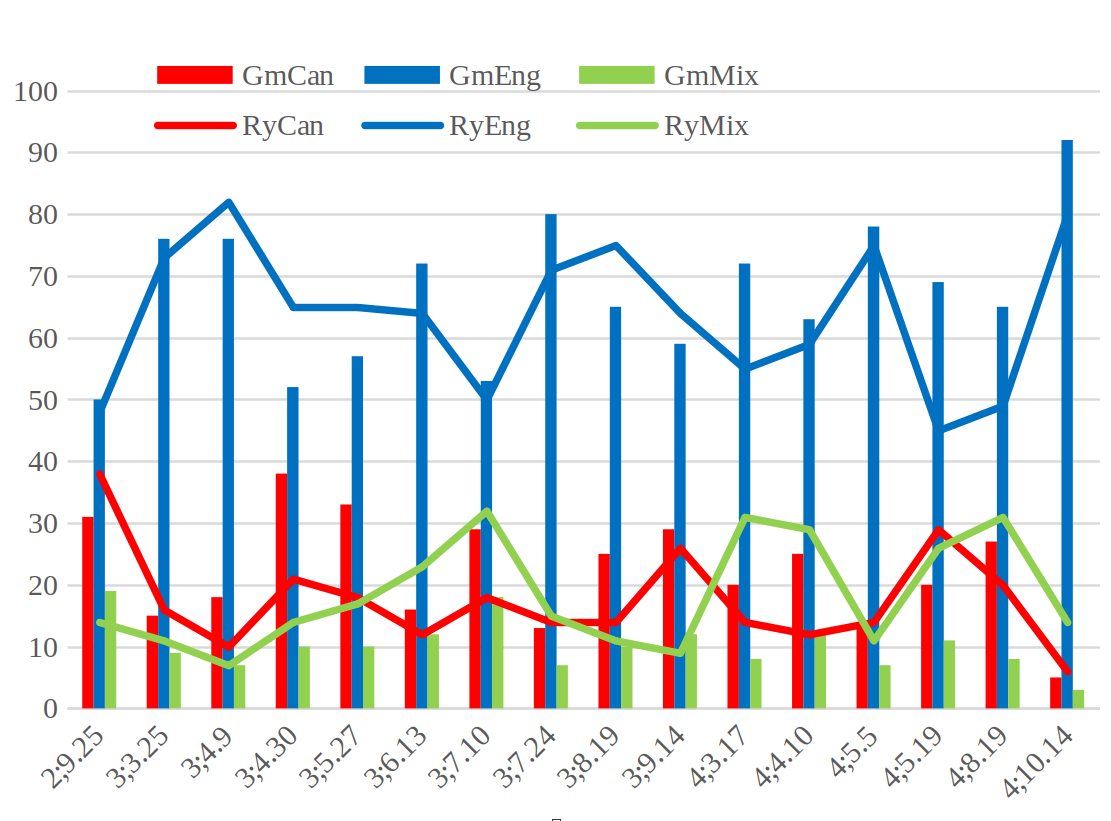
\includegraphics[width=\textwidth]{figures/quayfig1.png}

\caption{\label{fig:quay:1} Percentage of Cantonese, English and Mixed utterances in Grandmother’s input and Ryan’s output}
\end{figure}

\subsection{Intrasentential code-switching: Quantity and quality}\label{sec:quay:4.2}
\largerpage
Both had the lowest number and percentage of mixed utterances roughly matching in percentage for each type of intrasentential switching in \tabref{tab:quay:2}. Their mixed utterances were mostly one-word insertions into multiword utterances in the other language. Adding ENGchi and CHIeng utterances together, one-word insertions make up 69\% of PGM’s mixed utterances (n = 825) and 62\% of RYA’s (n = 439). The whole family always used Cantonese kinship terms to show respect for familial relationships and status based on gender and seniority by using  {specific terms such as \textit{maamaa} and \textit{yeye} for \textit{paternal} grandmother and grandfather, respectively. Thus, RYA had no choice but to use these Cantonese terms of address when speaking in English. They make up the bulk of one-word insertions in predominantly English utterances (ENGchi in \tabref{tab:quay:2}) for both PGM (64\%) and RYA (67\%) and are not truly intrasentential switches as they behave more like proper names that do not change.} They had the same proportion at 8\% of two-word mixed utterances such as: “kiss \textit{kumyong}” ‘like this’ (2;9.25); “\textit{pinkoh} ‘which-one’ driver” (3;7.10); “\textit{mou} ‘no’ ink” (4;5.19) from PGM, and “where \textit{dinwa}” ‘phone’ (2;9.25); “\textit{wakje} ‘perhaps’ yes” (4;3.17); “\textit{kum} ‘so’ small” (4;8.19) from RYA. The child did have a higher proportion of multiword mixed utterances at 30\% (211/709) than PGM at 23\% (269/1194). An example from RYA would be “this \textit{kiew chou} ‘(is) called’ dark blue” (3;5.27) while PGM’s example shows interclausal as well as intrasentential code-switching: “go inside here \textit{mei unwui chengtou teiha lo}” ‘so (you) don’t dirty (the) floor’ (3;3.25).

\begin{table}
\caption{Type of intrasentential code-switching by PGM (N = 1194) and RYA (N = 709) in 16 sessions}
\label{tab:quay:2}
\begin{tabularx}{\textwidth}{l@{~~}Yr@{~~}YYr@{~~}Y}
\lsptoprule
 &   & {PGM}  &  &  &  {RYA}   & \\
 \cmidrule(lr){2-4}\cmidrule(lr){5-7}
%\hhline%%replace by cmidrule{~------}
 {Type of intrasentential CS} & { \# of utts.} & \% &  {Kinship terms} & \# of utts. & \% &  {Kinship terms}\\
\midrule 
One-CHI word (ENGchi) &  222 &  19 &  \mbox{141 (64\%)} &  167 &  24 &  \mbox{112 (67\%)}\\
One-ENG word (CHIeng) &  603 &  51 &  &  272 &  38 & \\
Total one-word insertions & 825 & 69 &  & 439 & 62 & \\
TWOmix: two-word utts. & 100 & 8 &  & 59 & 8 & \\
ENG-CHI: multi-word utts. & 269 & { 23} &  & 211 & 30 & \\
\lspbottomrule
\end{tabularx}
\end{table}

\section{Discussion} %5. /

\subsection{Grandmother’s code-switching practices as support for the weaker language}\label{sec:quay:5.1}

The emergent bilingual child was pragmatically sensitive to the language choice of his grandmother despite his limited ability in English. From the early recordings onwards, RYA matched PGM’s English input with a similar proportion of English utterances (but see next section for \textit{qualitative} differences in the child’s English output).  \figref{fig:quay:1} and \tabref{tab:quay:2} showed that RYA was sensitive to PGM’s 89\% intersentential \textit{and} 11\% intrasentential code alternations. As he got older, she increased her English utterances.

The way PGM used English with Cantonese to support RYA’s English development is reminiscent of studies of classroom code-switching as outlined by Faltis (2019: 49, \tabref{tab:quay:2}.1). PGM provided English vocabulary and encouraged collaborative construction of meaning while she read to him. In Example \REF{ex:quay:1} from the first recording, she supplied translation equivalents and gave additional information in RYA’s stronger language to help him understand the weaker one (more Cantonese was used here than in later sessions). She scaffolds the story for her grandson by switching from English to Cantonese to provide translations, elaborate on the meaning of English utterances or confirm his comprehension. Her turns are long as she tries to reinforce the main ideas from the story and encourage discussion even though RYA responds (as at preschool) through actions rather than words. PGM’s Cantonese utterances are in italics with English glosses between single quotes and English insertions in predominantly Cantonese utterances underlined.

\setcounter{equation}{0}
\ea%1
    \label{ex:quay:1}
         PGM is reading from a book to RYA at age 2;9.25\\
1 *PGM:  There is a big cat there. Have you seen a cat? \textit{Nei tung ngo taiha} ‘have a look with me’. See \textit{kohko} ‘that’ cat. \textit{Nei tai keitoh} cat \textit{ah} ‘you (can) see so many cat(s)’. What is the cat doing? Huh? What is cat…what is \textit{yeye} ‘grandpa’ doing? What is \textit{yeye} doing? He is eating. You see this cat. One two. You see the eyes so big. You’ve got big eyes? How many cats here? Busy, busy kitties. What are they doing?\\
   *RYA:  0.\\
     \%act:  flips page\\
2 *PGM:  Kitty’s sitting. \textit{Huikeh tau kum chai lok hui} ‘(it) puts its head down like that’. \textit{Hui} \textit{wan ye hai yappin koh} box \textit{tou wan ye} ‘it’s looking for something inside the box’. \textit{Ikoh le} ‘what about this’? Kitty peeking. \textit{Chongchongchong} ‘(It’s) peeking’. \textit{Huikeh ngan kumyong chongchong} ‘its eyes are peeking like that’. \textit{Timyong chongchong} ‘how does (it) peek’?\\
   *RYA:  0.\\
     \%act:  opens eyes wide\\
3 *PGM:  Oh. And then this kitty \textit{hang lou} ‘walks along’. Strolling along. \textit{Ikoh le} ‘what about this’? Kitty rolling. Roll. \textit{Kumyong chuen chuen chuen} ‘roll roll roll like that’. \textit{Tai hui kumyong chuen chuen chuen hui keh} body ‘see how it rolls rolls rolls its body’. Kitty hissing. \textit{Kei auk eh hui ngau} ‘how fiercely it bites’. \textit{Huitit nga kei lei ah} ‘how sharp are its teeth’. Don’t go near a cat. Little kitten. \textit{Tai huikeh nga kei} sharp \textit{ah haimou} ‘its teeth are so sharp aren't they’? \textit{Ngau yan keh haimou} ‘it bites people doesn’t it’? \textit{Nei yat chengtou hui hui chau ngau neikeh sau kelo nei chimou} ‘do you know that if you offend it, it will bite your hand’? \textit{Ikoh} ‘this’ kitty kissing. Kissing kissing. \textit{Tai hui leongko} \textit{kiss kiss} \textit{haimou} ‘can you see that the two of them are kissing’? Kiss kiss. \textit{Nah ikoh} ‘here this’ kitty is running. \textit{Timyong chau ah} ‘how does it run’? \textit{Chau chau chau chau kumyong ah} ‘does it run run run run like this’?

    \%sit:  PGM pretends to run with downturned index and middle fingers along the sofa
\z

This example shows mainly intersentential codeswitches where the utterances are English-only or Cantonese-only (the code-switching pattern recommended for teachers in \citealt{Faltis2019}). Eight utterances exemplify intrasentential codeswitches with four depicting one-word English insertions (“cat”, “box”, “body” and “sharp”) into otherwise Cantonese utterances that describe what can be seen in the book. The remaining four code-mixed utterances are: “See \textit{kohko} ‘that’ cat”, “\textit{Ikoh} ‘this’ kitty kissing”, “\textit{Tai hui leongko} ‘see the two of them’ kiss kiss \textit{haimou} ‘right’”, “\textit{Nah ikoh} ‘here this’ kitty is running”. The Cantonese insertions are demonstratives (and deictic) to encourage the child to look at the pictures while the story is commented on in English. In turn 1, the English word “cat” is repeated eight times as the main topic of the book, followed by its synonym “kitty”, used in subsequent turns. PGM associates the actions depicted in the book to the grandfather’s action of eating in the same room and compares RYA’s eyes to the cat’s eyes. In turn 2 after the child turns the page, she explains the English word “peeking” in Cantonese. When asked in Cantonese how the cat peeks, RYA shows his understanding by opening his eyes wide. In turn 3, PGM provides translation equivalents for “strolling” and “rolling” to explain the actions of the cat. For “hissing”, she explains in Cantonese why a cat would hiss and uses the opportunity to warn against disturbing cats who may bite. She does not provide a Cantonese equivalent for “kissing” (a known word) but does so for “running”, supplementing it by running her fingers along the sofa they are sitting on. PGM unconsciously and inadvertently supports her grandson’s emergent bilingualism using the same types of cues and practices \citet{Faltis2019} has outlined for classroom code-switching practices by teachers. \citet{AntónEtAl2016} also found that language mixing in the classroom during concept acquisition is not detrimental to learning outcomes.

PGM often switched to Cantonese while reading books in English whenever RYA offered comments in Cantonese, thus encouraging and engaging him to interact in whichever language he preferred. The child generally accommodated his grandmother’s language choice patterns proportionally. Interestingly, striking similarities in code-switching patterns as shown in \figref{fig:quay:1} and \tabref{tab:quay:2} were also found from corpus data of bilingual adults and developing bilingual children from the same community.  \citet[74]{PhillipsDeuchar2021} suggest that their corpus findings support a usage-based approach whereby children “are acquiring the [code-switching] patterns of speech produced in the input available to them” as depicted in this case study.

\subsection{Qualitative differences between the emergent bilingual child’s English and Cantonese utterances}\label{sec:quay:5.2}

What is surprising from the quantitative analyses is that this child who hardly spoke any English at preschool did so with his grandmother from the earliest session, and in general, matched his grandmother’s language choices. Despite similar code-switching patterns to his grandmother, qualitative analyses show that his English utterances were much shorter and more limited in morphosyntactic structure than his Cantonese utterances. Until almost age five, most of his English utterances were: one-word nouns referring to animals, food or objects as depicted in books; various short phrasal utterances like “no more paper”, “all finished”, or “up the ladder”; or full or partial repetitions of his grandmother’s English utterances. He was often asked to repeat English words in the preschool setting, and PGM did the same explicitly at home, for example at age 3;4.9, in “Big hug \textit{nei kong la}” (‘you say (it)’). All such utterances and some set phrases like “I don’t know”, “I don’t remember”, and “Wait a minute” inflated his English total. Towards age five, he produced a few spontaneous short sentences like: “I see this”, “I think it’s a worm”, “I found it”, “I rolled six”, “Six is the biggest number”. His longest English utterances occurred when singing songs like “Old MacDonald had a farm” or when reciting the alphabet or counting aloud.

Despite accommodating his grandmother’s use of English from the first session, RYA was dominant in Cantonese, which is not obvious from the quantitative analyses. \tabref{tab:quay:3} lists 20 examples of his typical Cantonese utterances during the preschool period to show that in contrast to his English utterances, his Cantonese utterances were well-formed sentences with finite verbs from Session 1. The last column provides literal translations into English with parentheses around English elements not in the original Cantonese to show congruence where possible (when needed, a better English gloss is provided after the equal symbol between parentheses, and square brackets surround additional contextual information not expressed in original examples). Numbered examples in Cantonese are preceded by C in \tabref{tab:quay:3}, Mixed ones by M in \tabref{tab:quay:4}, and English examples by E in \tabref{tab:quay:5}.

A brief description of Cantonese grammar is necessary. Cantonese, like other Chinese dialects, is a pro-drop language with very little of the grammatical morphology prominent in English, such as inflectional markings of person, gender, case, number (except for pronouns), tense or mood (\citealt{MatthewsYip2011}). Indeed, Cantonese has few affixes compared to English; its grammatical relationships are mainly encoded by relative word position and strict adherence to word order. Like English, its basic word order is SVO (subject-verb-object) as in C4, C8–9, C17–18 in \tabref{tab:quay:3}. But unlike English, the following deviations are possible: \REF{ex:quay:1} SOV as in C12; \REF{ex:quay:2} V + S order or subject-verb inversion; \REF{ex:quay:3} right-dislocation where an element is put last or added separately from the rest of the sentence (as in M5, \tabref{tab:quay:4}); and \REF{ex:quay:4} topicalization (as in M6). Because Cantonese is a topic-prominent language, it has a more flexible word order than English since various elements of a sentence can become the sentence topic by being placed first (\citealt{MatthewsYip2011}). Implicit subjects are identified by pragmatic-discourse criteria from the immediate speech context and discourse topic \citep{LukeEtAl2003}. This is evident from examples C2, C3, C5–7, C10, C14–16, and C20. While every sentence must have a subject in English, this is not required in Cantonese as indicated by the parentheses surrounding overt subjects in English translations of RYA’s Cantonese (\tabref{tab:quay:3}) and ENG-CHI compound/complex utterances (\tabref{tab:quay:4}). The subject pronoun can be retrieved from the immediate speech context as for C6 which RYA said while looking at a turkey being roasted in the oven. In C15, he is at the table with PGM when he refers to how the alphabet letters he is writing extends to where his grandmother is sitting. The preposition (PREP) \textit{hai} in C4 and C5 function like verbs and can occur in a sentence on its own without a verb as in those two examples. RYA’s well-formed Cantonese utterances conveyed his intentions clearly as when he told PGM in C9 that he would change his pants after spilling water on himself or in C4 at 2;9.25 when he informed PGM that he would fetch a toy telephone for them to play with. C17 and C20 have the aspect marker (ASP) indicating past tense.


\begin{table}[b!]
\caption{Examples of Ryan’s Cantonese utterances}
\small
\label{tab:quay:3}
\begin{tabularx}{\textwidth}{ll>{\raggedright}p{25mm}Q}
\lsptoprule
\textbf{Age} (Sess. \#) & \textbf{Ex} & \textbf{Cantonese} & \textbf{Literal} \textbf{translations} (ENG elements absent in CAN in parentheses)\\
\midrule
2;9.25 (1) & C1 & \textit{Itit um nau nau nau nau.} & This (does) not bite bite bite bite.\\
          & C2 & \textit{Yap umtuk hui.} & Inside can’t go (=(It) can’t go in).\\
          & C3 & \textit{Um pei chueyfan.} & (You are) not allowed to cook.\\
          & C4 & \textit{Ngo lo tinwa hai kohtou.} & I bring the telephone PREP (from) there.\\
\tablevspace
3;4.9 (4) & C5 & \textit{Chung yau ye hai yappin.} & Still more things PREP inside (it) (=There are) more things inside).\\
      & C6 & \textit{Oi chuey dou hui hui um yuk tuk.} & (You) must cook PRT (until [turkey]) can’t move. \\
      & C7 & \textit{Tit zo yap hui.} & (It) fell inside.\\
      & C8 & \textit{Ngo um oi tuk.} & I (do) not want to read (it).\\
\tablevspace
3;7.24 (8) & C9 & \textit{Ngo hui wun jek tiew foo.} & I (will) go (to) change (my) pants.\\
      & C10 & \textit{Lau pei shuey.} & drip nose water (=(I have a) runny nose).\\
      & C11 & \textit{Maamaa hui pintou?} & Grandma go where? (=where is Grandma going?)\\
      & C12 & \textit{Ijek yan mou chin mai.} & This person (does) no (=not-have) money (to) buy/spend.\\
\tablevspace
4;4.10 (12) & C13 & \textit{Hai meye ikoh?} & Is what this? (=What is this?)\\
      & C14 & \textit{Hai kum yong}. & (It) is like this.\\
      & C15 & \textit{Cheung tou maamaa kohtou.} & Long PREP (=[letters he’s writing] reaches) grandma over-there. \\
      & C16 & \textit{Kum hakmanman.} & (It’s) so dark.\\
\tablevspace
4;10.14 (16) & C17 & Ryan \textit{um kei tuk zo.} & Ryan (does) not remember ASP.\\
      & C18 & \textit{Maamaa tai um dou.} & Grandma (could) not see PRT.\\
      & C19 & \textit{Hai mai itou}? & Is-or-is-not (it) here?\\
      & C20 & \textit{Choh zo.} & Wrong ASP (=(It was) wrong)].\\
\lspbottomrule
\end{tabularx}
\end{table}

\largerpage
\tabref{tab:quay:3} does not show the production of all possible grammatical elements in Cantonese. For example, while PGM produced sentence-final particles (SFP) like \textit{la} in \textit{nei kong la} ‘you say (it)’ or \textit{lo} in lines 5–6 of Example \REF{ex:quay:3}, none appeared in RYA’s Cantonese utterances. RYA does have some prepositions (PREP in C4–5), particles (PRT in C6, C18) and aspect (ASP in C17, C20) markers. Note that Cantonese-speaking preschool children in Hong Kong also develop grammatical features at different rates according to age and individual factors \citep{Wong2023}.


\subsection{ {Discourse} {strategies} {in} {multi-word} {Mixed} {and} {English} {utterances} }\label{sec:quay:5.3}

Example \REF{ex:quay:2} is a typical dual-language conversation. At age 4;8.19, RYA is almost matching PGM here in number of turns (4RYA:5PGM) in contrast to 15 months earlier in Example \REF{ex:quay:1} (1RYA:3PGM). PGM asks the first question in Cantonese but the next two Cantonese questions contain a conjunction and proper name (of a shopping mall) in English. RYA then responds with a Cantonese deictic expression, \textit{kohko}, followed in English by the conjunction “and” with the mall’s name. In lines 5 to 12, when the conversation is relatively simple and straightforward, both PGM and RYA continue speaking in English. He answers his grandmother in line 9 with one rare full English sentence, “I like Metrotown too.” Line 11 (“Every sushi store”) is more typical of his short phrasal utterances in English, which his grandmother expands into a full sentence in line 12.

\ea%2
    \label{ex:quay:2}
         Ryan and his grandmother discuss which sushi places he likes at age 4;8.19 \\

1   *PGM:  \textit{Kumyat sushi housek mah} ‘was the sushi yummy today’? \\
2   *PGM:  Uh? \\
3   *PGM:  \textit{Nei chungyi kumyat sek kohkan} or \textit{chungyi hui} Metrotown \textit{sek kohkan} ‘do you like the place we ate at today or do you like the one at Metrotown’?\\
4   *RYA:   \textit{Kohko} ‘that one’ and Metrotown.\\
5   *PGM:   Both? \\
6   *PGM:  You also like today’s one? \\
7   *PGM:  Davie one [street name]. \\
8   *PGM:  You don’t like Metrotown?\\
9   *RYA:   I like Metrotown too.\\
10 *PGM:   Which one is better?\\
11 *RYA:   Every sushi store.\\
12 *PGM:   Every sushi store is good?\\
13 *RYA:   Metrotown upstair \textit{yau keh} ‘have that’ store. \\
14 *RYA:   Down \textit{hai} ‘is’ … upstair \textit{yau keh} ‘have that’ sushi place.\\
15 *RYA:  And down there \textit{yau} ‘have’...and and…up there \textit{yau} sushi place. \\
16 *RYA:  And down there \textit{yau} sushi place.\\
17 *PGM:   \textit{uh koh} ‘that’ foodcourt \textit{lo.} \\
18 *RYA:   \textit{yau} three, three sushi place.

    \z

He code-switched intrasententially when he needed to convey more complicated information (lines 13–16 and 18) about the location of three different Japanese restaurants in the mall. Sharing the same background knowledge of the layout of the mall, PGM understood him even though his elaborations consist of Cantonese verbal elements with seemingly truncated noun and prepositional phrases in English. 

Combining English and Cantonese in multiword utterances is the child’s typical discourse strategy to extend the messages he can convey. Notably, his multiword ENG-CHI utterances were the longest, comprising 30\% of all his intrasentential code-switched utterances (n = 211, \tabref{tab:quay:2}). Although his Cantonese-only utterances were simple sentences, some of his multiword \textit{mixed} utterances were complex sentences (with coordinate or subordinate clauses) due to congruent lexicalization, an issue rarely discussed (as mentioned earlier) in the literature on children’s code-switching \citep{Treffers-Daller2022}. \citeauthor{Muysken1997} (\citeyear{Muysken1997,Muysken2000}), in describing this type of code-switching for adults, explained that it occurs when two languages share grammatical structures that can be filled lexically with elements from~either language. Example \REF{ex:quay:3} shows that RYA produced an 11-word ENG-CHI utterance equivalent in English to a complex sentence with a subordinating conjunction in line 4:

\ea%3
    \label{ex:quay:3}
         Reading a book at age 3;4.9 \\
1 *PGM:  E for?\\
2 *RYA:  Egg.\\
3 *PGM:  Oh, and it is cracking.\\
4 *RYA:  baby \textit{nganngan tuk chut lei tai teiha yau mou mama} birdie ‘the baby [bird] is looking out to see if its mother birdie is on the ground’.\\
5 *PGM:  \textit{hai lo} ‘yes’. \\
6 *PGM:  \textit{tai hui mama hai tou mou lo} ‘it is checking if its mother is around’.

    \z
Predominantly Cantonese mixed utterances as in line 4 above were much longer than predominantly English mixed utterances. While RYA produced more English words in Example \REF{ex:quay:2} at 4;8.19 (lines 13–16, 18), the insertion of verbs in Cantonese indicates a reliance on Cantonese morphosyntactic structure. While \textit{yau} ‘have’ was used the most often, other Cantonese verbs often inserted into English utterances are \textit{hai} ‘is/copula’, \textit{hui} ‘go’, \textit{kiew} ‘is called’ and \textit{pei} ‘give’. Cantonese verb insertions helped the child to produce relatively long English utterances early on:

\ea%4
    \label{ex:quay:4}
         Looking at alphabet flashcards at age 3;4.9\\
1 *RYA:  And \textit{yau} ‘have’ one two three flower in there.\\
2 *PGM:  Three flowers. Wow. That’s good.
    \z

Pointing out three flowers on the flashcard, he inserts English words into a Cantonese framework where ‘there’ occurs at the end as in \textit{yau yat yi sam-go faa hai godou} and not at the beginning as it would in an English utterance. Although PGM models the plural inflection of “flower” in line 2, RYA’s lack of plural marking is also a sign of congruent lexicalization as his more established Cantonese system does not require such inflections nor subject pronouns.  

\tabref{tab:quay:4} lists 11 examples from 54 recordings (including the 16 sessions used earlier) of ENG-CHI complex and compound utterances that provide evidence that: \REF{ex:quay:1} English elements are superimposed on Cantonese structures (i.e., congruent lexicalization), and \REF{ex:quay:2} bilingual mixed utterances are much longer than unilingual English or Cantonese utterances. Although limited, the hybrid examples in \tabref{tab:quay:4} indicate congruent lexicalization and convergence occurring. For example, in M1, the English insertions fit the dependent clause preceding the independent one conveyed by ‘when this one is finished, I will use blue’ (referring to the ink in coloring pens). Both clauses, however, are derived from Cantonese verbs – \textit{mou sai} ‘to be finished’ does not require the subordinating conjunction (when) and \textit{jung} ‘use’ does not require a subject pronoun. Thus, “this one \textit{mou saai zau jung} blue” is an example of the way \citet{Clyne2003} defined convergence as a hybrid form that exhibits elements from two linguistic systems. The final column contains literal translations of the ENG-CHI utterances with parentheses around elements absent in Cantonese. If all the English insertions are translated directly into Cantonese from M1–M7 and M9–M11, he would have well-formed Cantonese utterances. For example, in relating how he won a game of Snakes \& Ladders, RYA’s English insertion of “number and then win” in M3 is a direct translation from Cantonese of \textit{souzi tungmaai jengzo} that follows after \textit{houdo} ‘a lot of’ without the plural inflection on “number”, without the first-person subject pronoun (I) or past tense inflection (albeit the irregular “won”), all of which are not required in Cantonese and reflected in his English lexical insertions. M8 is the only example that does not share complete word-order congruence in the two languages as the placement of “more” follows the English order after ‘a little’ rather than coming before in Cantonese as in \textit{ngo zing do siusiu}. The subordinating conjunction \textit{mai} ‘so that’ is followed by the English verb “make” with a Cantonese direct object in the same way as a literal Cantonese translation \textit{[choudou] houdo chin}.  \citet[277]{Gawlitzek-MaiwaldTracy2005} proposed that “convergence comes about when children (assisted by universal grammar) reconstruct derivational relationships linking hitherto independent systems” and that this gives us insights into children’s early awareness of cross-linguistic equivalence and contrasts. The child used this transitional strategy for more than a year from M1 to M11 because his grandmother never failed to understand him. For example, M7 was produced when he asked his grandmother about a book with text he had seen previously but could not find that day. She told him the book had already been returned to the library. Her response conveyed to him the acceptability of his code-mixing pattern which did not impede their meaningful communication.

Although PGM modelled mixed utterances, she produced a smaller proportion at 11\% versus RYA at 19\% (\figref{fig:quay:1}) and decreased such utterances greatly through adherence to intersentential code-switching by the last recording while RYA’s intrasentential code-switching increased. Only in the last session does he produce three English-based mixed utterances with one-word Cantonese insertions as shown below (excluding the kinship term in b), indicating perhaps the start of a shift in his Cantonese dominance (although M11 in \tabref{tab:quay:4} still shows Cantonese verbs supporting predominantly English utterances). He produces:

\ea
ENGchi utterances at 4;10.14\\
    \ea I think Ryan roll \textit{zo}.
    \ex Ryan move \textit{zo} \textit{maamaa} down.
    \ex How Ryan try the red one \textit{yausi}?
    \z
\z

\begin{table}
\caption{The child’s ENG-CHI utterances beyond simple sentences}
\label{tab:quay:4}
\small
\begin{tabularx}{\textwidth}{llQQ}
\lsptoprule
\textbf{Age}  & \textbf{Ex} & \textbf{ENG-CHI} (or Mix beyond one-word insertions) & \textbf{Literal} \textbf{translations} (ENG elements absent in CAN in parentheses)\\
\midrule
3;5.27 & M1 & This one \textit{mou saai zau jung} blue. & (When) this one (is) \textit{finished} (I will) \textit{use} blue.\\
3;9.28 & M2 & How \textit{yeye chou} chair \textit{tai} tv and then Ryan \textit{dyeu bei yeye hai} chair. & How(-about) \textit{grandpa sit(s) on} (the) chair (to) \textit{watch} TV and then Ryan \textit{throws} [toy] \textit{to grandpa on} (the) chair.\\
4;1.23 & M3 & \textit{Gumjat} Ryan \textit{houdo} number and then win. & \textit{Today} Ryan (had) (a) \textit{lot of} number(s) and then (I won).\\
4;2.13 & M4 & \textit{Maamaa} \textit{hai mai} Ryan \textit{jau} nine and then go up the ladder? & \textit{Grandma is-or-is-not} (that when) Ryan \textit{gets} nine and then go(es) up the ladder?\\
4;3.17 & M5 & \textit{Heoi go godou sin} turn remember? & \textit{After we reach there}, (we) turn, remember?\\
4;4.17 & M6 & Ryan two year old \textit{ngo lei} and then \textit{cheng lan hai mai}? & (When) Ryan (was) two year(s) old \textit{I came} and then \textit{broke} (it) \textit{didn’t} (I)?\\
4;4.10 & M7 & \textit{Maamaa} how come last time \textit{jau go} book \textit{hai godou jau} word \textit{se hai godou.} & \textit{Grandma}, how come last time \textit{there was} (a) book (and there) \textit{were} word(s) \textit{written there.}\\
4;7.30 & M8 & \textit{Ngo zing siusiu} more \textit{mai} make \textit{houdo chin.} & \textit{I make a little} more \textit{so that} (I can) make \textit{lots of money.} [inverted: little more=\textit{do} \textit{siusiu}]\\
4;7.30 & M9 & How [Ryan] push this up and then \textit{yeye} \textit{faaidit} \textit{se.} & How(-about) Ryan push this up and then grandpa hurry (to) shoot.\\
4;8.19 & M10 & How \textit{maamaa sai zo wun maamaa tung ngo waan} snake and ladder? & How(-about) [when] \textit{grandma finish(es)} \textit{washing} (the) \textit{dishes}, \textit{grandma play(s)} snake(s) and ladder(s) \textit{with me.}\\
4;10.14 & M11 & \textit{Hai} fifty-seven plus twelve \textit{mai} sixty nine? & \textit{Is} (it) fifty-seven plus twelve (that) \textit{make(s)} sixty nine?\\
\lspbottomrule
\end{tabularx}
\end{table}

The past tense of English verbs is indicated by the Cantonese aspect marker \textit{zo} ‘already’ rather than with an ‘-ed’ inflection in a and b. He also used the split order of the verb-particle (“move down”), preferred in English but not in Cantonese. \citet[12]{YipMatthews2016} considered this an innovation when their Cantonese-dominant children in Hong Kong produced the split order in Cantonese-based mixed utterances not found in the adult Cantonese input. Likewise, a and b are an innovative use of congruent lexicalization for RYA in Canada with English as the base for Cantonese insertions since PGM never used \textit{zo} with an English verb but did produce it as expected with Cantonese verbs in mixed utterances like “The boat \textit{lan zo} ‘is broken’” (i.e., qualitatively different from RYA’s mixing). In c, the utterance is mostly English except for the Cantonese adverb \textit{yausi} (‘again’), indicating an emerging English proficiency.

RYA’s well-formed Cantonese utterances (\tabref{tab:quay:3}) provide evidence of his language dominance which influenced not only English insertions in ENG-CHI complex/compound utterances (\tabref{tab:quay:4}) but also the production of unilingual English utterances. Previous studies have focused on code-mixed utterances without examining utterances produced in a single code. If we accept that the child is using his stronger language to support his weaker one through congruent lexicalization, we can examine convergence or hybridity in his spontaneously produced English utterances. As mentioned earlier, very few of his English utterances contained subjects and predicates. Most of his two-or-more-word ENG utterances appear to be ungrammatical in English when analyzed according to English grammatical rules but not when analyzed according to Cantonese grammatical rules. \tabref{tab:quay:5} shows 20 such \textit{ungrammatical} English examples translated into Cantonese. The literal Cantonese translations with pro-drop/subject omission in E1–5, E9–11, E19–20 show that the English utterances were based on the morphosyntactic structure of Cantonese (see \citealt{Wong2023} for more on Cantonese grammar). Unlike the Hong Kong bilingual child who was also Cantonese-dominant in \citet{YipMatthews2000}, RYA always produced \textit{wh}{}-words like \textit{what} (E6), \textit{where} (E12) and \textit{how} (E13, 16, 19) consistently in initial position as required in English but not in Cantonese, a \textit{wh}{}-in-situ language where \textit{wh} words may serve as a subject or an object \citep{Wong2023}. This interrogative construction may be more salient in English exposure in Canada than in Hong Kong and was the only one where RYA did not transfer Cantonese structure into his English utterances.

\begin{table}
\small
\caption{Examples of Ryan’s English utterances}
\label{tab:quay:5}
\begin{tabularx}{\textwidth}{lllQ}
\lsptoprule
\textbf{Age}  (Sess. \#) & \textbf{Ex} & \textbf{English}  & [= \textbf{literal} \textbf{CAN} \textbf{translation}]: English meaning\\
\midrule
2;9.25 \REF{ex:quay:1} & E1 & No this one. & [=Umhai ikoh]: ‘(it’s) not this one’.\\
          & E2 & Wash like this. & [=Sai kumyeong]: ‘(I) wash (it) like this’.\\
          & E3 & Stir chocolate. & [=Gaao zyugulik]: ‘(I) stir (the) chocolate’.\\
          & E4 & Water right. & [=Sui haimai]: ‘(it’s) water, isn’t it?’\\
3;4.9 (4) & E5 & Two flower. & [=Loenggo faa]: ‘(there’s) two flower(s)’.\\
          & E6 & What behind? & [=Houmin meye]: ‘what (is) behind?’\\
          & E7 & There two. & [=Godou loenggo]: ‘there (is) two (of them)’.\\
          & E8 & This one ghost. & [=Jigo gwai]: ‘this-one (is a) ghost’.\\
3;7.24 (8) & E9 & How down hill? & [=Dim loksaan]: ‘How (do I go) down (the) hill?’\\
          & E10 & How down the tail? & [=Dim lokheoi tiu mei]: ‘How (do I go) down (the) tail?’\\
          & E11 & Go up the ladder. & [=Soeng lautai]: ‘(I) go up (the) ladder’.\\
          & E12 & Where the paddle? & [=Syun joeng bindou]: ‘where (is the) paddle?’ \\
4;4.10 (12) & E13 & How about this one? & [=Jigo dim]: meaning ‘how (is) this one?’\\
          & E14 & This one two\textbf{s}. & [=Jigo leong go]: ‘this one (has) two (of them)’.\\
          & E15 & This one back too. & [=Jigo dou faanlei]: ‘this one (is) turned around’.\\
          & E16 & How this one? & [=Jigo dim]: ‘how (is) this one?’\\
4;10.14 (16) & E17 & Down the snake. & [=Lok gogo se]: ‘(I go) down that snake’\\
          & E18 & More there. & [=Godou zungyau]: ‘(there’s) more there’.\\
          & E19 & How now? & [=jigaa dim]: ‘how (is it) now?’\\
          & E20 & How change color? & [=dim wun ngaansik]: ‘how (do I) change color?’\\
\lspbottomrule
\end{tabularx}

\end{table}

Although Cantonese and English are not closely related, both share a basic SVO structure that facilitated the transfer of the morphosyntactic frame of RYA’s stronger language, Cantonese, into his English utterances, resulting in examples of congruent lexicalization and convergence in Tables 4 and 5. This was not apparent until English utterances were translated back into Cantonese. Thus, the surface English elements mask the underlying Cantonese morphosyntactic rules used in their construction, exemplifying clearly how separate languages can no longer be identified and are only “discernible after the fact; that is, convergence is an outcome (of borrowing or substratum influence, for instance) and not an observable process” (\citealt{BullockToribio2004}: 91). This use of hybrid morphosyntactic forms as translingual practice gives the child time to develop his English ability and acquire target English structures without compromising meaningful communication with his bilingual grandmother. His English grammar does develop over time with the production of articles and plural inflections in later sessions. For example, “Stir chocolate” (E3) lacks a definite article unnecessary in Cantonese that is produced later at 3;7.24 in E10–12 and E17; “Two flower” (E5) shows no plural inflection but a plural marking appears, albeit erroneously, in “This one twos” (E14). As mentioned earlier, prepositions in Cantonese can function like verbs and can occur in sentences on their own without verbs. This flexible usage of prepositions is exemplified with the preposition ‘down’ in E9–10, and E17 (also seen earlier in Example \REF{ex:quay:2}, lines 14–16). Although their results were based on \textit{visible} code-switching, Yow et al. (2018: 1085; their emphasis) conclude in their study of preschool children in Singapore that “the ACT of code-switching by children may have provided them with a way to engage both their languages more frequently, particularly the weaker language.” Code-switching also allowed the Singaporean children to improve their developing bilingual proficiency as it does for RYA. Although PGM’s utterances and RYA’s utterances were qualitatively different, no breakdown in communication ever occurred, thus emphasizing that dual language use in the home was a \textit{fluid} bilingual practice that gave the emergent bilingual child time to develop his weaker language.

\section{Conclusion}\label{sec:quay:6}

Examining the child’s code-switching practices revealed his abilities rather than the deficiencies often highlighted by the monolingual-normed understanding of proficiency subscribed to by schools and society. The grandmother socialized the child into using his whole linguistic repertoire to express himself fully by modelling dual-language usage that made it acceptable for the child to produce mixed utterances. As a result of such bilingual interactions, the child was able to accommodate to his grandmother’s use of English. Unlike his grandmother’s data, he used congruent lexicalization (\citeauthor{Muysken1997} \citeyear{Muysken1997,Muysken2000}) and convergence (\citealt{BullockToribio2004, Clyne2003, Toribio2004}) as part of his code-switching practices: \REF{ex:quay:1} to convey information in longer mixed complex/compound sentences beyond the simple sentences of unilingual utterances, and \REF{ex:quay:2} to form complete utterances in his weaker language by using the morphosyntactic rules of his stronger language. Both types of code-switching strategies where the child arranged English-only and English-mixed utterances according to Cantonese morphosyntactic rules reflect hybridity. This study reveals the need for researchers to examine not just intrasentential mixed utterances in future studies but also \textit{unilingual} utterances in the weaker language where the code-mix through convergence may be invisible. The child in this study capitalizes on the structural congruence between his two languages. He uses congruent lexicalization and convergence as part of his strategy to accommodate his grandmother’s use of English as well as insertion and language alternation that more clearly demarcate his two languages. RYA’s use of congruent lexicalization/convergence in his code-switching practice provides evidence not only that his Cantonese system is stronger than his English system but that he can use bilingual bootstrapping (\citealt{Gawlitzek-MaiwaldTracy1996}) and cross-linguistic lexical and structural equivalence to increase the production of his weaker language. This mixing/hybrid pattern reveals also what the child may perceive as more versus less advanced options as his weaker language catches up with the stronger one in development. What is unclear is whether longitudinal empirical data can indicate how he distinguishes his coexisting structural formats from coexisting grammars and where he draws the limit between these options. That is, when does his strategy of convergence yield to two distinct systems? This is not apparent from the data set used for this study. In personal communication with the child’s mother, it appears that RYA was assessed by his school around age 6;6 as on a par with monolingual English peers, which suggests that his grandmother’s code-switching practices helped him to transition faster from the home to the school language.

Case studies like this one are valuable (despite their obvious limitations) because they can refute generalizations, show what is possible, and give rise to hypotheses (as explained in \citealt{DeucharQuay2001}). This study refutes the generalization that emergent bilinguals are producing \textit{broken} English when they enter school. The hybrid nature of RYA’s English utterances (in his use of congruent lexicalization and convergence) indicate child agency because despite limited English ability, he used his available linguistic resources to match his grandmother’s language choice. Indeed, the child produced a similar proportion of English-only utterances tp his grandmother from the outset and could form much longer complex/compound sentences when he could draw on his two languages. From a methodological viewpoint, this case study reveals that code-switching research should not just focus on dual-language utterances but also on single-language utterances that appear ungrammatical in a weaker language since convergence as a substratum influence may not be observable at the surface-level of the utterance (\citealt{BullockToribio2004}). That is, English utterances can be analyzed not only with English grammar rules but also with the grammar of children’s stronger language to consider whether congruency allows that grammar to be used as a base for the weaker language. 

This study has implications not only for raising bilingual children at home using code-switching input but also for the treatment of emergent bilinguals in the school setting. Primary school teachers need to appreciate that children can draw upon linguistic resources from their HLs to develop a weaker school language and not view emergent bilinguals as linguistically deficient. Emergent bilinguals or English language learners (ELLs) are expected to make up 25\% of school-aged children in the US by 2025 (\citealt{NationalEducationAssociation2020}) with many natively-born rather than newcomers (\citealt{ZongBatalova2015}). More research is needed to address the dilemma mentioned earlier of when and how to introduce the societal language without compromising HL maintenance, which  \citet[345]{WongFillmore1991} states is related to “timing, not English” adding that the “children have to learn English, but they should not be required to do so until their native languages are stable enough to handle the inevitable encounter with English and all it means.” Three decades after that exhortation, we still do not know when an HL can be considered stable enough for it to survive when these children start English medium education. Clearly, legitimizing HL identity and changing attitudes toward an acceptance of hybrid language practices for ELLs would encourage and validate the maintenance of HLs in English-speaking countries.

\section*{Acknowledgment}

I am enormously grateful to the child’s parents and extended family for being a part of this case study, but especially to PGM and RYA, without whom this study would not have been possible. Thanks are also due to Janice Nakamura and Sheung Yu Cheung for their assistance with the transcriptions, coding, and translations. I am also indebted to the anonymous reviewer whose extensive comments helped greatly to reshape the focus of this chapter.
\sloppy\printbibliography[heading=subbibliography,notkeyword=this]
\end{document}
